\documentclass[a4paper]{article}

\def\npart {IV}
\def\nterm {Lent}
\def\nyear {2018}
\def\nlecturer {A.\ J.\ Scholl}
\def\ncourse {Topics in Number Theory}

% Imports
\ifx \nextra \undefined
  \usepackage[pdftex,
    hidelinks,
    pdfauthor={Dexter Chua},
    pdfsubject={Cambridge Maths Notes: Part \npart\ - \ncourse},
    pdftitle={Part \npart\ - \ncourse},
  pdfkeywords={Cambridge Mathematics Maths Math \npart\ \nterm\ \nyear\ \ncourse}]{hyperref}
  \title{Part \npart\ - \ncourse}
\else
  \usepackage[pdftex,
    hidelinks,
    pdfauthor={Dexter Chua},
    pdfsubject={Cambridge Maths Notes: Part \npart\ - \ncourse\ (\nextra)},
    pdftitle={Part \npart\ - \ncourse\ (\nextra)},
  pdfkeywords={Cambridge Mathematics Maths Math \npart\ \nterm\ \nyear\ \ncourse\ \nextra}]{hyperref}

  \title{Part \npart\ - \ncourse \\ {\Large \nextra}}
\fi

\author{Lectured by \nlecturer \\\small Notes taken by Dexter Chua}
\date{\nterm\ \nyear}

\usepackage{alltt}
\usepackage{amsfonts}
\usepackage{amsmath}
\usepackage{amssymb}
\usepackage{amsthm}
\usepackage{booktabs}
\usepackage{caption}
\usepackage{enumitem}
\usepackage{fancyhdr}
\usepackage{graphicx}
\usepackage{mathtools}
\usepackage{microtype}
\usepackage{multirow}
\usepackage{pdflscape}
\usepackage{pgfplots}
\usepackage{siunitx}
\usepackage{tabularx}
\usepackage{tikz}
\usepackage{tkz-euclide}
\usepackage[normalem]{ulem}
\usepackage[all]{xy}

\pgfplotsset{compat=1.12}

\pagestyle{fancyplain}
\lhead{\emph{\nouppercase{\leftmark}}}
\ifx \nextra \undefined
  \rhead{
    \ifnum\thepage=1
    \else
      \npart\ \ncourse
    \fi}
\else
  \rhead{
    \ifnum\thepage=1
    \else
      \npart\ \ncourse\ (\nextra)
    \fi}
\fi
\usetikzlibrary{arrows}
\usetikzlibrary{decorations.markings}
\usetikzlibrary{decorations.pathmorphing}
\usetikzlibrary{positioning}
\usetikzlibrary{fadings}
\usetikzlibrary{intersections}
\usetikzlibrary{cd}

\newcommand*{\Cdot}{\raisebox{-0.25ex}{\scalebox{1.5}{$\cdot$}}}
\newcommand {\pd}[2][ ]{
  \ifx #1 { }
    \frac{\partial}{\partial #2}
  \else
    \frac{\partial^{#1}}{\partial #2^{#1}}
  \fi
}

% Theorems
\theoremstyle{definition}
\newtheorem*{aim}{Aim}
\newtheorem*{axiom}{Axiom}
\newtheorem*{claim}{Claim}
\newtheorem*{cor}{Corollary}
\newtheorem*{defi}{Definition}
\newtheorem*{eg}{Example}
\newtheorem*{fact}{Fact}
\newtheorem*{law}{Law}
\newtheorem*{lemma}{Lemma}
\newtheorem*{notation}{Notation}
\newtheorem*{prop}{Proposition}
\newtheorem*{thm}{Theorem}

\renewcommand{\labelitemi}{--}
\renewcommand{\labelitemii}{$\circ$}
\renewcommand{\labelenumi}{(\roman{*})}

\let\stdsection\section
\renewcommand\section{\newpage\stdsection}

% Strike through
\def\st{\bgroup \ULdepth=-.55ex \ULset}

% Maths symbols
\newcommand{\bra}{\langle}
\newcommand{\ket}{\rangle}

\newcommand{\N}{\mathbb{N}}
\newcommand{\Z}{\mathbb{Z}}
\newcommand{\Q}{\mathbb{Q}}
\renewcommand{\H}{\mathbb{H}}
\newcommand{\R}{\mathbb{R}}
\newcommand{\C}{\mathbb{C}}
\newcommand{\Prob}{\mathbb{P}}
\renewcommand{\P}{\mathbb{P}}
\newcommand{\E}{\mathbb{E}}
\newcommand{\F}{\mathbb{F}}
\newcommand{\cU}{\mathcal{U}}
\newcommand{\RP}{\mathbb{RP}}
\newcommand{\CP}{\mathbb{CP}}

\newcommand{\ph}{\,\cdot\,}

\DeclareMathOperator{\sech}{sech}
\DeclareMathOperator{\cosech}{cosech}
\DeclareMathOperator{\cosec}{cosec}

\DeclareMathOperator{\covol}{covol}
\DeclareMathOperator{\vol}{vol}

\let\Im\relax
\let\Re\relax
\DeclareMathOperator{\Im}{Im}
\DeclareMathOperator{\Re}{Re}
\DeclareMathOperator{\im}{im}
\DeclareMathOperator{\image}{image}
\DeclareMathOperator{\Ann}{Ann}

\DeclareMathOperator*{\res}{res}
\DeclareMathOperator{\Res}{Res}
\DeclareMathOperator{\Ind}{Ind}

\DeclareMathOperator{\tr}{tr}
\DeclareMathOperator{\diag}{diag}
\DeclareMathOperator{\rank}{rank}
\DeclareMathOperator{\card}{card}
\DeclareMathOperator{\spn}{span}
\DeclareMathOperator{\adj}{adj}

\DeclareMathOperator{\erf}{erf}
\DeclareMathOperator{\erfc}{erfc}

\DeclareMathOperator{\ord}{ord}
\DeclareMathOperator{\Sym}{Sym}

\DeclareMathOperator{\sgn}{sgn}
\DeclareMathOperator{\orb}{orb}
\DeclareMathOperator{\stab}{stab}
\DeclareMathOperator{\ccl}{ccl}

\DeclareMathOperator{\lcm}{lcm}
\DeclareMathOperator{\hcf}{hcf}

\DeclareMathOperator{\Int}{Int}
\DeclareMathOperator{\id}{id}

\DeclareMathOperator{\betaD}{beta}
\DeclareMathOperator{\gammaD}{gamma}
\DeclareMathOperator{\Poisson}{Poisson}
\DeclareMathOperator{\binomial}{binomial}
\DeclareMathOperator{\multinomial}{multinomial}
\DeclareMathOperator{\Bernoulli}{Bernoulli}
\DeclareMathOperator{\like}{like}

\DeclareMathOperator{\var}{var}
\DeclareMathOperator{\cov}{cov}
\DeclareMathOperator{\bias}{bias}
\DeclareMathOperator{\mse}{mse}
\DeclareMathOperator{\corr}{corr}

\DeclareMathOperator{\otp}{otp}
\DeclareMathOperator{\dom}{dom}

\DeclareMathOperator{\Root}{Root}
\DeclareMathOperator{\supp}{supp}
\DeclareMathOperator{\rel}{rel}
\DeclareMathOperator{\Hom}{Hom}
\DeclareMathOperator{\Aut}{Aut}
\DeclareMathOperator{\Gal}{Gal}
\DeclareMathOperator{\Mat}{Mat}
\DeclareMathOperator{\End}{End}
\DeclareMathOperator{\Char}{char}
\DeclareMathOperator{\ev}{ev}
\DeclareMathOperator{\St}{St}
\DeclareMathOperator{\Lk}{Lk}
\DeclareMathOperator{\disc}{disc}
\DeclareMathOperator{\Isom}{Isom}
\DeclareMathOperator{\length}{length}
\DeclareMathOperator{\energy}{energy}
\DeclareMathOperator{\area}{area}
\DeclareMathOperator{\Syl}{Syl}
\DeclareMathOperator{\cl}{cl}
\DeclareMathOperator{\fix}{fix}

\newcommand{\GL}{\mathrm{GL}}
\newcommand{\SL}{\mathrm{SL}}
\newcommand{\PGL}{\mathrm{PGL}}
\newcommand{\PSL}{\mathrm{PSL}}
\newcommand{\PSU}{\mathrm{PSU}}
\newcommand{\Or}{\mathrm{O}}
\newcommand{\SO}{\mathrm{SO}}
\newcommand{\U}{\mathrm{U}}
\newcommand{\SU}{\mathrm{SU}}

\renewcommand{\d}{\mathrm{d}}
\newcommand{\D}{\mathrm{D}}

\tikzset{->/.style = {decoration={markings,
                                  mark=at position 1 with {\arrow[scale=2]{latex'}}},
                      postaction={decorate}}}
\tikzset{<-/.style = {decoration={markings,
                                  mark=at position 0 with {\arrowreversed[scale=2]{latex'}}},
                      postaction={decorate}}}
\tikzset{<->/.style = {decoration={markings,
                                   mark=at position 0 with {\arrowreversed[scale=2]{latex'}},
                                   mark=at position 1 with {\arrow[scale=2]{latex'}}},
                       postaction={decorate}}}
\tikzset{->-/.style = {decoration={markings,
                                   mark=at position #1 with {\arrow[scale=2]{latex'}}},
                       postaction={decorate}}}
\tikzset{-<-/.style = {decoration={markings,
                                   mark=at position #1 with {\arrowreversed[scale=2]{latex'}}},
                       postaction={decorate}}}

\tikzset{circ/.style = {fill, circle, inner sep = 0, minimum size = 3}}
\tikzset{mstate/.style={circle, draw, blue, text=black, minimum width=0.7cm}}

\definecolor{mblue}{rgb}{0.2, 0.3, 0.8}
\definecolor{morange}{rgb}{1, 0.5, 0}
\definecolor{mgreen}{rgb}{0.1, 0.4, 0.2}
\definecolor{mred}{rgb}{0.5, 0, 0}

\def\drawcirculararc(#1,#2)(#3,#4)(#5,#6){%
    \pgfmathsetmacro\cA{(#1*#1+#2*#2-#3*#3-#4*#4)/2}%
    \pgfmathsetmacro\cB{(#1*#1+#2*#2-#5*#5-#6*#6)/2}%
    \pgfmathsetmacro\cy{(\cB*(#1-#3)-\cA*(#1-#5))/%
                        ((#2-#6)*(#1-#3)-(#2-#4)*(#1-#5))}%
    \pgfmathsetmacro\cx{(\cA-\cy*(#2-#4))/(#1-#3)}%
    \pgfmathsetmacro\cr{sqrt((#1-\cx)*(#1-\cx)+(#2-\cy)*(#2-\cy))}%
    \pgfmathsetmacro\cA{atan2(#2-\cy,#1-\cx)}%
    \pgfmathsetmacro\cB{atan2(#6-\cy,#5-\cx)}%
    \pgfmathparse{\cB<\cA}%
    \ifnum\pgfmathresult=1
        \pgfmathsetmacro\cB{\cB+360}%
    \fi
    \draw (#1,#2) arc (\cA:\cB:\cr);%
}
\newcommand\getCoord[3]{\newdimen{#1}\newdimen{#2}\pgfextractx{#1}{\pgfpointanchor{#3}{center}}\pgfextracty{#2}{\pgfpointanchor{#3}{center}}}

\def\Xint#1{\mathchoice
   {\XXint\displaystyle\textstyle{#1}}%
   {\XXint\textstyle\scriptstyle{#1}}%
   {\XXint\scriptstyle\scriptscriptstyle{#1}}%
   {\XXint\scriptscriptstyle\scriptscriptstyle{#1}}%
   \!\int}
\def\XXint#1#2#3{{\setbox0=\hbox{$#1{#2#3}{\int}$}
     \vcenter{\hbox{$#2#3$}}\kern-.5\wd0}}
\def\ddashint{\Xint=}
\def\dashint{\Xint-}

\DeclareMathOperator\Br{Br}
\renewcommand\G{\hat{\mathbb{G}}}
\newcommand\A{\mathbb{A}}
\begin{document}
\maketitle
{\small
\setlength{\parindent}{0em}
\setlength{\parskip}{1em}
The ``Langlands programme'' is a far-ranging series of conjectures describing the connections between automorphic forms on the one hand, and algebraic number theory and arithmetic algebraic geometry on the other. In these lectures we will give an introduction to some aspects of this programme.

\subsubsection*{Pre-requisites}
The course will follow on naturally from the Michaelmas term courses \emph{Algebraic Number Theory} and \emph{Modular Forms and L-Functions}, and knowledge of them will be assumed. Some knowledge of algebraic geometry will be required in places.
}
\tableofcontents

\setcounter{section}{-1}
\section{Introduction}
In this course, we shall first give an outline of class field theory. We then look at abelian $L$-functions (Hecke, Tate). We then talk about \emph{non-}abelian $L$-functions, and in particular the Weil--Deligne group and local $L$- and $\varepsilon$-factors.

We then talk about local Langlands for $\GL_n$ a bit, and do a bit of global theory and automorphic forms at the end.

The aim is not to prove everything, because that will take 3 courses instead of one, but we are going to make precise definitions and statements of everything.

\section{Local Class field theory}
\subsection{Preliminaries}
Class field theory is the study of abelian extensions of local or global fields.
\begin{notation}
  Let $K$ be a field. We will write $\bar{K}$\index{$\bar{K}$} for a separable closure of $K$, and $\Gamma_K = \Gal(\bar{K}/K)$\index{$\Gamma_K$}. We have
  \[
    \Gamma_k = \lim_{L/K\text{ finite separable}} \Gal(L/K),
  \]
  which is a \term{profinite group}. The associated topology is the \term{Krull topology}.
\end{notation}

Galois theory tells us
\begin{thm}[Galois theory]
  There are bijections
  \begin{align*}
    \left\{\parbox{3cm}{\centering closed subgroups of $\Gamma_K$}\right\} &\longleftrightarrow \left\{\parbox{3cm}{\centering subfields $K \subseteq L \subseteq \bar{K}$}\right\}\\
    \left\{\parbox{3cm}{\centering open subgroups of $\Gamma_K$}\right\} &\longleftrightarrow \left\{\parbox{3cm}{\centering finite subfields $K \subseteq L \subseteq \bar{K}$}\right\}
  \end{align*}
\end{thm}

\begin{notation}
  We write \term{$K^{ab}$} for the maximal abelian subextension of $\bar{K}$, and
  \[
    \Gal(K^{ab}/K) = \Gamma_K^{ab} = \frac{\Gamma_K}{\overline{[\Gamma_K, \Gamma_K]}}.
  \]
\end{notation}
Note that $\bar{K}$ is unique, but only up to non-canonical isomorphism. Indeed, it has many automorphisms, given by elements of $\Gal(\bar{K}/K)$. Thus, $\Gamma_K$ is well-defined up to conjugation only. Thus, $\Gamma_K^{ab}$ is well-defined.

Let $F$ be a \term{non-archimedean local field}\index{local field}, i.e.\ either a finite extension of $\Q_p$, or $\F_q((t))$. This has a normalized valuation $v = v_F: F^\times \twoheadrightarrow \Z$, and we have a \term{valuation ring} $\mathcal{O} = \mathcal{O}_F$. We pick some uniformizer $\pi = \pi_F$, which is an element with $v(\pi) = 1$. We write\index{$k$}\index{$k_F$}
\[
  k = k_F = \text{residue field} \cong \F_q,\quad q = p^r.
\]
Inside $F^{ab}$, we have \term{$F^{ur}$}, the \term{maximal unramified extension} of $F$. We have the Galois group
\[
  \Gamma_F \supseteq I_F = \Gal(\bar{F}/F^{ur}) \supseteq P_F,
\]
where \term{$I_F$} is the \term{inertia group}, and \term{$P_F$} is the \term{wild inertia group}, i.e.\ the maximal pro-$p$-subgroup of $I_F$.

Unramified extensions are classified by extensions of the residue field, and the reduction map gives an isomorphism
\[
  \Gamma_F/I_F \cong \Gal(\bar{k}/k) \cong \hat{\Z} = \lim_{n \geq 1} \Z/n\Z.
\]
where \term{$\hat{Z}$} is the profinite completion of $\Z$.

Inside $\Gal(\bar{k}/k)$, we have the \term{arithmetic Frobenius} $\varphi_q: x \mapsto x^q$. If we decide to identify $1 \in \hat{\Z}$ with $\varphi_q$, that is going to lead to infinite confusion. Instead, we define $\Frob_q = \varphi_q^{-1}$\index{$\Frob_q$}, which we call the \term{geometric Frobenius}. We fix $\Gal(\bar{k}/k) \cong \hat{\Z}$ by setting $1$ to be $\Frob_q$.

The reason this is called the geometric Frobenius is that if we have a scheme over a finite field, then there are two ways the Frobenius can act on it --- either as a Galois action, or as algebraic map given by pulling back along the $q$th power map. The latter is the geometric one.

Now that we understand $\Gamma_F/I_F$, we want to give a description of $I_F/P_F$. For $n$ prime to $p$, fix $\pi_n \in \bar{F}$ with $\pi_n^n = \pi$. We define
\begin{align*}
  t(n): I_F = \Gal(\bar{F}/F^{ur}) &\to \mu_n(\bar{k}) = \{\zeta \in \bar{k}: \zeta^n =1 \}\\
  \gamma &\mapsto \gamma(\pi_n)/\pi_n\pmod \pi.
\end{align*}
This is the \term{tame mod $n$ character}. Note that since $\gamma$ fixes $\pi = \pi_n^n$, this indeed maps to the right place, and does not depend on the choices. It follows that this is a homomorphism $I_F \to \mu_n(\bar{k})$.

Consider the limit over all $n$ to obtain a map
\[
  I_F \to \lim_{(n, p) = 1} \mu_n(\bar{k}) = \prod_{\ell \not= p} \lim_{m \geq 1} \mu_{\ell^m}(\bar{k}) \equiv \prod_{\ell \not= p} \Z_{\ell}(1)(\bar{k}).
\]
This \term{$\Z_{\ell}(1)(\bar{k})$} is the \term{Tate module} of $\bar{k}^{\times}$. This is isomorphic to $\Z_{\ell}$, but not canonically.

So we have a map $\hat{t} \prod_{\ell \not= p} t_\ell$. The main theorem is that
\begin{prop}
  $\ker \hat{t} = P_F$.
\end{prop}
This means the maximal tamely ramified extension of $F$ is
\[
  \bigcup_{(n, p) = 1} F^{ur} (\sqrt[n]{\pi}).
\]
The map $\hat{t}$ is just Kummer theory.

Note that $t(n)$ extends to a map $\Gamma_F \to \mu_n$ given by the same formula, but it is not a homomorphism, because
\[
  t(n)(\gamma \delta) = \frac{\gamma\delta(\pi_n)}{\pi_n} = \frac{\gamma(\pi_n)}{\pi_n} \gamma \left(\frac{\delta(\pi_n)}{\pi_n}\right) = t(n)(\gamma) \cdot \gamma(t(n)(\delta)).
\]
If $\gamma$ is in the inertia group, $\gamma$ acts trivially, but this is not true in general. So this formula just says that $t(n)$ is a $1$-cocycle. This \emph{does} depend on the choices
\subsection{Local class field theory}
Local class field theory is often stated in terms of finite extensions, but it makes more sense to work with infinite extensions.
\begin{thm}[Local class field theory]\index{local class field theory}
  There exists a unique family of continuous homomorphisms, the \term{local Artin map}\index{$\Art_F$}\index{Artin map!local}
  \[
    \Art_F: \to \Gamma_F^{ab}
  \]
  with dense image characterized by
  \begin{enumerate}
    \item The following diagram commutes:
      \[
        \begin{tikzcd}
          F^{\times} \ar[d, two heads, "v_F"] \ar[r, "\Art_F"] & \Gamma_F^{ab} \ar[r, two heads] & \Gamma_F/I_F \ar[d, "\sim"]\\
          \Z \ar[rr, hook] & & \hat{\Z}
        \end{tikzcd}
      \]
    \item If $F'/F$ is finite, then
      \[
        \begin{tikzcd}
          (F')^\times \ar[r, "\Art_{F'}"] \ar[d, "N_{F'/F}"] & \Gamma_{F'}^{ab} = \Gal(F'^{ab}/F') \ar[d, "\text{restriction}"]\\
          F^\times \ar[r, "\Art_F"] & \Gamma_F^{ab} = \Gal(F^{ab}/F)
        \end{tikzcd}
      \]
  \end{enumerate}
  Moreover, $\Art_F^{-1}$ induces a bijection
  \[
    \left\{\parbox{4cm}{\centering open finite index\\subgroups of $F^\times$}\right\} \longleftrightarrow \left\{\parbox{4cm}{\centering open subgroups of $\Gamma_F^{ab}$}\right\}
  \]
  Of course, open subgroups of $\Gamma_F^{ab}$ further corresponds to finite abelian extensions of $F$. This is called the \term{existence theorem}

  Finally, if $F = \Q_p$ and $x = p^n y \in \Q_p^\times$ and $y \in \Z_p^\times$, then
  \[
    F^{ab} = \Q_p(\mu_\infty) = \bigcup \Q_p(\mu_n) = \Q_p^{ur} (\mu_{p^\infty}).
  \]
  Then
  \[
    \Art_\Q(x)|_{\Q_p^{ur}} = \Frob_p^n,\quad \Art_\Q(x) |_{\Q_p(\mu_{p^\infty})} = (\zeta_{p^n} \mapsto \zeta_{p^n}^{y \text{ mod }p^n}).
  \]
\end{thm}
If we had the arithmetic Frobenius instead, then we would have a $-y$ in the power there, which is less pleasant.

On the level of finite Galois extensions $E/F$, we can rephrase the first part of the theorem as giving a map
\[
  \Art_{E/F}: \frac{F^\times}{N_{E/F}(E^\times)} \to \Gal(E/F)^{ab}
\]
which is an isomorphism.

Finally, $\Art_F$ induces an isomorphism
\[
  \Q_F^\times \overset{\sim}{\to} \im(I_F \to \Gamma_F^{ab})
\]
and this maps $(1 + \pi \mathcal{O}_F)^\times$ to the image of $P_F$. Of course, the quotient $\mathcal{O}F^\times/(1 + \pi \mathcal{O}_F)^\times \cong k^\times = \mu_\infty(k)$.

Finally, this is functorial, namely if we have an isomorphism $\alpha: F \overset{\sim}{\to} F'$ and extend it to $\bar{\alpha} \bar{F} \overset{\sim}{\to} \to \bar{F}'$, then this induces isomorphisms between the Galois groups $\alpha_*: \Gamma_F \overset{\sim}{\to} \Gamma_{F'}$ (up to conjugacy), and $\alpha_*^{ab} \circ \Art_F = \Art_{F'} \circ \alpha_*^{ab}$.

The Artin map is not surjective. To fix this problem, it is convenient to introduce the \emph{Weil group}.
\begin{defi}[Weil group]\index{Weil group}
  The \emph{Weil group} of $F$ is a topological group $W_F$ defined as follows:
  \begin{itemize}
    \item As a group, it is
      \[
        W_F = \{\gamma \in \Gamma_F \mid \gamma|_{F^{ur}} = \Frob_q^n\text{ for some }n \in \Z\}.
      \]
      Recall that $\Gal(F^{ur}/F) = \hat{\Z}$, and we are requiring $\gamma|_{F^{ur}}$ to be in $\Z$. In particular, this contains $I_F$.
    \item The topology is defined by the property that $I_F$ is an \emph{open} subgroup with the profinite topology. So $W_F$ is a fiber product of topological groups
      \[
        \begin{tikzcd}
          W_F \ar[r, hook] \ar[d, two heads] & \Gamma_F \ar[d, two heads]\\
          \Z \ar[r, hook] & \hat{\Z}
        \end{tikzcd}
      \]
      where $\Z$ has the discrete topology.
  \end{itemize}
\end{defi}
Note that $W_F$ is not profinite. It is totally disconnected but not compact.

This seems like a slightly artificial definition, but this is cooked up precisely so that
\begin{prop}
  $\Art_F$ induces an \emph{isomorphism} of topological groups
  \[
    \Art_F^W: F^\times \to W_F^{ab}.
  \]
  This maps $\mathcal{O}_F^\times$ isomorphically onto the inertia subgroup of $\Gamma_F^{ab}$.
\end{prop}

We are not going to prove local class field theory, but we shall say something about the proof. There are three main methods:
\begin{itemize}
  \item The cohomological method (see Artin--Tate, Cassels--Fr\"ohlich), which only treats the first part, namely the existence of $\Art_K$. We start off with a finite Galois extension $E/F$, and we want to construct an isomorphism
    \[
      \Art_{E/F}: F^\times/N_{E/F}(E^\times) \to \Gal(E/F)^{ab}.
    \]
    Writing $G = \Gal(E/F)$, this uses the cohomological interpretation
    \[
      F^\times/N_{E/F}(E^\times) = \hat{H}^0(G, E^\times),
    \]
    where $\hat{H}$ is the Tate cohomology of finite groups. On the other hand, we have
    \[
      G^{ab} = H_1(G, \Z) = \hat{H}^{-2}(G, \Z).
    \]
    The main step is to compute
    \[
      H^2(G, E^\times) = \hat{H}^2(G, E^\times) \cong \frac{1}{n}\Z/\Z \subseteq \Q/\Z = H^2(\Gamma_F, \bar{F}^\times).
    \]
    where $n = [E:F]$. The final group $H^2(\Gamma_F, \bar{F}^\times)$ is the \term{Brauer group} $\Br(F)$, and the subgroup is just the kernel of $\Br(F) \to \Br(E)$.

    Once we have done this, we then define $\Art_{E/F}$ to be the cup product with the generator of $\hat{H}^2(G, E^\times)$, and this maps $\hat{H}^{-2}(G, \Z) \to \hat{H}^0(G, E^\times)$. The fact that this map is an isomorphism is rather formal.

    The advantage of this method is that it generalizes to duality theorems about $H^*(G, M)$ for arbitrary $M$, but this map is not at all explicit, and is very much tied to abelian extensions.
  \item Formal group methods: We know that the maximal abelian extension of $\Q_p$ is obtained in two steps --- we can write
    \[
      \Q_p^{ab} = \Q_p^{ur}(\mu_{p^\infty}) = \Q_p^{ur} (\text{torsion points in }\G_m),
    \]
    where $\hat{\G}_m$ is the formal multiplication group, which we can think of as $(1 + \mathfrak{m}_{\bar{\Q}_p})^\times$. This generalizes to any $F/\Q_p$ --- we have
    \[
      F^{ab} = F^{ur}(\text{torsion points in }\G_\pi),
    \]
    where $\G_\pi$ is the ``Lubin--Tate formal group''. This is described in Iwasawa's book, and also in a paper of Yoshida's. The original paper by Lubin and Tate is also very readable.

    The advantage of this is that it is very explicit, and when done correctly, gives both the existence of the Artin map and the existence theorem. This also has a natrual generalization to non-abelian extensions. However, it does not give duality theorems.
  \item Neukrich's method: Suppose $E/F$ is abelian and finite. If $g \in \Gal(E/F)$, we want to construct $\Art_{E/F}^{-1}(g) \in F^\times/N_{E/F}(E^\times)$. The point is that there is only one possibility, because $\bra g\ket$ is a cyclic subgroup of $\Gal(E/F)$, and corresponds to some cyclic extension $\Gal(E/F')$, and
    \begin{lemma}
      There is a finite $K/F'$ such that $K \cap E = F'$, so $\Gal(KE/K) \cong \Gal(E/F') = \bra g\ket$. Moreover, $KE/K$ is unramified.
    \end{lemma}
    Let $g'|_E = g$, and suppose $g' = \Frob_{KE/K}^a$. If local class field theory is true, then we have to have
    \[
      \Art_{KE/K}^{-1}(g') = \pi_K^a\pmod{N_{KE/K}(KE^\times)}.
    \]
    Then by our compatibility conditions, this implies
    \[
      \Art_{E/F}^{-1}(g) = N_{K/F}(\pi_K^a) \pmod {N_{E/F}(E^\times)}.
    \]
    The problem is then to show that this does not depennd on the choices, and then show that it is a homomorphism. These are in fact extremely complicated. Note that everything so far is just Galois theory. Solving these two problems is then where all the number theory goes in.
  \item When class field theory was first done, we first did \emph{global} class field theory, and deduced the local case from that. No one does that anymore nowadays, since we now have purely local proofs. However, when we try to generalize to the Langlands programme, we do not have any purely local way of doing so.
\end{itemize}

The Archimedean picture is not so interesting. There are only two Archimedean local fields, namely $\R$ and $\C$.
\begin{itemize}
  \item The Weil group of $\C$ is defined to be $W_\C = \C^\times$, and the Artin map $\Art^W_\R$ is defined to be the identity. $\Gamma_\C = \{1\}$.
  \item The Artin map $\Art_\R: \R^ \times \to \Gamma_\R^{ab} = \Gal(\C/\R) = \Z/2\Z$ is given by the sign. The Weil group is defined the non-abelian group
    \[
      W_\R = \bra \C^\times , \sigma \mid \sigma^2 = -1 \in \C^\times, \sigma z \sigma^{-1} = \bar{z}\text{ for all }z \in \C^\times\ket.
    \]
    This is a (non)-split extension of $\C^\times$ by $\Gamma_\R$,
    \[
      1 \to \C^\times \to W_\R \to \Gamma_\R \to 1,
    \]
    where in the last map, $z \mapsto 0$ and $\sigma \mapsto 1$. This is in fact the unique non-split extension of $\Gamma_\R$ by $\C^\times$ where $\Gamma_\R$ acts on $\C^\times$ in a natural way.

    There is also a Weil form of the Artin map, whose inverse is given by
    \begin{align*}
      (\Art_\R^W)^{-1}: W_\R^{ab} &\overset{\sim}{\to} \R^\times\\
      z &\mapsto z \bar{z}\\
      \sigma &\mapsto -1
    \end{align*}
\end{itemize}

These definitions seem very ad hoc, but they are not. To see this, we need to talk about the realtive Weil groups.
\begin{defi}[Relative Weil group]\index{relative Weil group}
  Let $F$ be a non-Archimedean field, and $E/F$ Galois but not necessarily finite. We define
  \[
    W_{E/F} = \{\gamma \in \Gal(E^{ab}/F) : \gamma|_{F^{ur}} = \Frob_q^n, n \in \Z\} = \frac{W_F}{\overline{[W_E, W_E]}}.
  \]
  with the quotient topology.
\end{defi}

The $W_{\bar{F}/F} = W_F$, while $W_{F/F} = F^\times$ by local class field theory.

Now if $E/F$ is a finite extension, then we have an exact sequence of Galois groups
\[
  \begin{tikzcd}
    1 \ar[r]& \Gal(E^{ab}/E) \ar[r] & \Gal(E^{ab}/F) \ar[r] & \Gal(E/F) \ar[r] \ar[d, equals]& 1\\
    1 \ar[r] & W_E^{ab} \ar[r] \ar[u, hook] & W_{E/F} \ar[r] \ar[u, hook] & \Gal(E/F) \ar[r] & 1.
  \end{tikzcd}
\]
By the Artin map, $W_E^{ab} = E^\times$. So the relative Weil group is an extension of $\Gal(E/F)$ by $E^\times$. In the case of Archimedean fields, we have
\[
  \lim_E E^\times \{1\}.
\]
So $\bar{F}^\times$ is invisible in $W_F = \lim W_{E/F}$. So the weirdness above comes from the fact that the separable closures of $\R$ and $\C$ are finite extensions. Observe that the extension above is characterized by an element of $H^2(\Gal(E/F), E^\times) \simeq \frac{1}{n}\Z/\Z$, and it is in fact $\frac{1}{n}$. We see that this is true also in the case of $\R$.

\subsection{Global class field theory}
Let $K$ be a global field, i.e.\ a number field or $k(C)$ for a smooth projective absolutely irreducible curve $C/\F_q$, i.e.\ a finite extension of $\F_q(t)$. It is possible to treat both of these cases the same way, but we are really only interested in the number field case.

Let \term{$\Sigma_K$} be the set of \term{places} of $K$, in the case of a number field this is the union $\Sigma_{K, \infty} \coprod \Sigma_K^\infty$, where \term{$\Sigma_{K, \infty}$}, the \term{infinite places} is the set of complex embeddings into $\C$ up to complex conjugation, and \term{$\Sigma_{K}^\infty$}, the \term{finite places} is the set of prime ideals of $\mathcal{O}_K$. We will call places $v, w, \ldots$. In the case of function fields, $\Sigma_K$ is just the set of closed points of $C$, or equivalently, the orbits of $C(\bar{\F_q})$ under the absolute Galois group. We write $v \mid \infty$ if $v$ is an infinite place, and $v \not \mid \infty$ otherwise.

If $v \in \Sigma_K$ is a place, there is a completion $K \hookrightarrow K_v$, where $K_v$ is $\R$ or $\C$ if $v \mid \infty$, and $K_v$ is a non-archimedean local field otherwise.

\begin{eg}
  If $\Q = K$, then there is one infinite prime, which we write as $\infty$, and we have the embedding $\Q \hookrightarrow \R$. If $v = p$, then we have the embedding $\Q \hookrightarrow \Q_p$ into the $p$-adic completion.
\end{eg}

\begin{notation}
  If $v$ is a finite place, we write $\mathcal{O}_v \subseteq K_v$ for the valuation ring of the completion.
\end{notation}

It is convenient to normalize our absolute values of $p$-adic fields. For doing class field theory, the right way of normalizing is as follows: we have $K_v \supseteq \mathcal{O}_v \supseteq \pi_v \mathcal{O}_v$, where $\pi_v \in K$ with $\pi_v \mathcal{O}_v$ the maximal ideal. The normalized valuation $v$ satisfies $v(\pi_v) = 1$. We have
\[
  q_v = \left|\frac{\mathcal{O}_v}{\pi_v \mathcal{O}_v}\right|.
\]
We then define
\[
  |x|_v = q_v^{-v(x)}.
\]
If $K = \Q$ and $v = p$, then $q_v = p$, and $|p|_v = \frac{1}{p}$.

In the Archimedean case, if $K_v$ is real, then we set $|x|$ to be the usual absolute value; if $K_v$ is complex, then we take $|x|_v = x\bar{x} = |x|^2$.

The reason for choosing these normalizations is that we have the following product formula:
\begin{prop}[Product formula]\index{product formula}
  If $x \in K^\times$, then
  \[
    \prod_{v \in \Sigma_K} |x|_v = 1.
  \]
\end{prop}
This is certainly true for $\Q$, and the general case is obtained by bootstrapping this from $\Q$.

\subsection{Adeles and ideles}
\begin{defi}[Adele]\index{adele}\index{$\mathbb{A}_K$}
  The \emph{adeles} is defined to be the restricted product
  \[
    \A_K = \prod_v' K_V = \left\{ (x_v)_v : \prod_v K_v : \text{ for all but finitely many $v \in \Sigma_K^\infty$, $x_v \in \mathcal{O}_v$}\right\}.
  \]
  We write this as $K_\infty \times \hat{K}$ or $\A_{K, \infty} \times \A_K^\infty$, where
  \[
    K_\infty = \A_{K, \infty} = K\otimes_\Q \R = \R^{r_1} \times \C^{r_2}.
  \]
  consists of the product over the infinite places, and
  \[
    \hat{K} = \A_K^\infty = \prod_{v \nmid \infty}' \bigcup_{\text{finite }S \subseteq \Sigma_K^\infty} \prod_S K_V \times \prod_{v \in \Sigma_K^\infty \setminus S} \mathcal{O}_V.
  \]
  This contains $\hat{\mathcal{O}}_K = \prod_{v \nmid \infty} \mathcal{O}_K$. In the case of a number field, $\hat{\mathcal{O}}_K$ is the profinite completion of $\mathcal{O}_K$. More precisely, if $K$ is a number field then
  \[
    \hat{\mathcal{O}}_K = \lim \frac{\mathcal{O}_K}{\mathfrak{a}} = \lim \mathcal{O}_K/N\mathcal{O}_K = \mathcal{O}_K \otimes_\Z \hat{\Z},
  \]
  where the last equality follows from the fact that $\mathcal{O}_K$ is a finite $\Z$-module.
\end{defi}
%When adeles was first invented, they used the normal product instead of the restricted product, and it turned out to be a terrible idea, since taking the product of infinitely many copies of $\Z$'s lying inside each $K_V$ gives you something ghastly.

\begin{defi}[Idele]\index{idele}\index{$J_K$}\index{$\mathbb{A}_K^\times$}
  The \emph{ideles} is the restricted product
  \[
    J_K = \A_K^\times = \prod_v' K_v^\times = \{(x_v \in \prod K_v^\times: \text{for almost all }v, x_v \in \mathcal{O}_v^\times\}.
  \]
\end{defi}
This looks really horrible, but it is actually pretty finite because of the topology we have on it. We take $K_\infty \times \hat{\mathcal{O}}_K$ to be an open subgroup with the product topology. Once we have done this, there is a unique structure of a topological ring for which this holds. On $J_K$, we take $K_\infty^\times \times \hat{\mathcal{O}}_K^\times$ to be open with the product topology. Note that this is not the subspace topology under the inclusion $J_K \hookrightarrow \A_K$. Instead, it is induced by the inclusion
\begin{align*}
  J_K &\hookrightarrow \A_K \times \A_K\\
  x &\mapsto (x, x^{-1})
\end{align*}
It is a basic fact that $K^\times \subseteq J_K$ is a \emph{discrete} subgroup. The \term{idele class group} is then
\[
  C_K = J_K/K^\times.
\]
$J_K$ comes with a natural absolute value
\begin{align*}
  |\ph|_A: J_K &\to \R_{> 0}^\times\\
  (x_v) &\mapsto \prod_{v \in \Sigma_K} |x_v|_v.
\end{align*}
The product formula implies that $|K^\times|_{\A} = \{1\}$. So this in fact a map $C_K \to \R_{>0}^\times$.

\begin{thm}
  The map $|\ph|_\A: C_K \to \R_{>0}^\times$ has compact kernel.
\end{thm}
This theorem is equivalent to the finiteness of class number and Dirichlet's unit theorem.

\begin{eg}
  In the case $K = \Q$, we have
  \[
    J_{\Q} = \R^\times \times \prod'_p \Q_p^\times.
  \]
  Suppose we have an idele $x = (x_v)$. It is easy to see that there exists a unique rational number $y \in \Q^\times$ such that $\sgn(y) = \sgn(x_\infty)$ and $v_p(y) = v_p(x_p)$. So we have
  \[
    J_\Q = \Q^\times \times \left(\R^\times_{>0} \times \prod_p \Z_p^\times\right).
  \]
  Here we think of $\Q^\times$ as being embedded diagonally. So $\Q^\times$ is discrete. So
  \[
    C_\Q = \R_{>0}^\times \times \hat{\Z}^\times,
  \]
  and $\hat{\Z}^\times$ is the kernel $|\ph|_{\A}$.
\end{eg}

Now consider the subgroup $\R^\times_{>0} \subseteq \C_\Q$. This is the maximal connected subgroup of $C_\Q$, and is in fact the intersection of all open subgroups containing $1$. In general, we can define
\[
  \pi_0(C_K) = C_K/C_K^0,
\]
where $C_K^0$ is the maximal connected subgroup. Then
\[
  \pi_0(C_\Q) = \hat{\Z}^\times = \lim_n (\Z/n\Z)^\times = \lim_n \Gal(\Q(\zeta_n)/\Q) = \Gal(\Q(\zeta_\infty)/\Q).
\]
In fact, $\Q(\zeta_\infty)$ is the maximal abelian extension of $\Q$. Global class field theory is a generalization of this isomorphism to all fields.

Suppose $L/K$ is a finite Galois extension, and a place $v$ of $K$, and a place $w \mid v$ of $L$. For finite places, this means the corresponding primes divide; for infinite places, this means the embedding $w$ is an extension of $v$. We then have the \term{decomposition group}
\[
  \Gal(L_w/K_v) \subseteq \Gal(L/K).
\]
If $L/K$ is abelian, since any two places lying above $v$ are conjugate, this depends only on $v$. In this case, we can now define the \term{global Artin map}\index{Artin map!global}
\[
  \Art_{L/K}: J_K \to \Gal(L/K)
\]
Note that if $x_v \in \mathcal{O}_v^\times$, where $L/K$ is unramified at $v \in \Sigma_K^\infty$, then the local Artin map $\Art_{K_w/K_v}(x_v) = 1$. So for an arbitrary idele, we can define
\[
  \Art_{L/K}((x_v)_v) = \prod_v \Art_{L_w/K_v} (x_v),
\]
where we pick one $w$ for each $v$. If we pass to the limit over extensions $L/K$, we get a continuous map
\[
  \Art_K : J_K \to \Gamma_K^{ab}.
\]
\begin{thm}[Artin reciprocity law]\index{Artin reciprocity law}\leavevmode
  $\Art_K(K^\times) = \{1\}$, so induces a map $C_K \to \Gamma_K^{ab}$. Moreover, $\Art_K$ induces isomorphisms of topological groups:
  \begin{enumerate}
    \item If $\Char(K) = p > 0$, then $\Art_K$ is injective, and induces an isomorphism $\Art_K: C_k \overset{\sim}{\to} W_K^{ab}$, where $W_K$ is defined just as in the local case. Since $K$ is a finite extension of $\F_q(T)$, and wlog assume $\bar{\F}_q \cap K = \F_q = k$. Then $W_K$ is defined as the pullback
      \[
        \begin{tikzcd}
          W_K \ar[r, hook] \ar[d] & \Gamma_K = \Gal(\bar{K}/K) \ar[d, "\mathrm{restr}."]\\
          \Z \ar[r, hook] & \hat{\Z} \cong \Gal(\bar{k}/k)
        \end{tikzcd}
      \]
    \item If $\char(K) = 0$, we have an isomorphism
      \[
        \Art_K: \pi_0(C_K) = \frac{C_K}{C_K^0} \overset{\sim}{\to} \Gamma_K^{ab}.
      \]
  \end{enumerate}
  Moreover, if $L/K$ is finite, then we have a commutative diagram
  \[
    \begin{tikzcd}
      C_L \ar[d, "N_{L/K}"] \ar[r, "\Art_L"] & \Gamma_L^{ab} \ar[d, "\mathrm{restr.}]\\
      C_K \ar[r, "\Art_K"] & \Gamma_K^{ab}
    \end{tikzcd}
  \]
  If this is in fact Galois, then this induces an isomorphism
  \[
    \Art_{L/K}: \frac{J_K}{K^\times N_{L/K}(J_L)} \overset{\sim}{\to} \Gal(L/K)^{ab}.
  \]
  Finally, this is functorial, namely if $\sigma; K \overset{\sim}{\to} K'$ is an isomorphism, then we have a commutative square
  \[
    \begin{tikzcd}
      C_K \ar[r, "\Art_K"] \ar[d, "\sigma"] & \Gamma_K^{ab} \ar[d]\\
      C_{K'} \ar[r, "\Art_{K'}] & \Gamma_{K'}^{ab}
    \end{tikzcd}
  \]
\end{thm}
Observe that naturality and functoriality are immediate consequences of the corresponding results for local class field theory.

As a consequence of the isomorphism, we know that we have a corresopndence
\begin{align*}
  \left\{\parbox{4cm}{\centering finite abelian extensions $L/K$}\} &\longleftrightarrow \left\{\parbox{4cm}{\centering open subgroups of finite index $J_K$ containing $K^\times$}\right\}\\
  L &\longmapsto \ker(\Art_{L/K}: J_K \to \Gal(L/K))
\end{align*}
Note that there exists finite index subgroups that are not open.

Let $L/K$ be abelian, and $U = \ker (\Art_{L/K}: J_K \to \Gal(L/K))$. Then from local class field theory, $L/K$ is unramified at $v \nmid \infty$ if $U \supseteq \mathcal{O}_v^\times$.

If $v \mid \infty$ is real, we say $v$ is ramified for some (and hence for all) places $w$ of $L$ above $v$, $w$ is complex (Neukirch would say $v$ is inert). Then $L/K$ is unramified at a real place $v$ iff $U \supseteq K_v^\times = \R^\times$. Note that since $U$ is open, it automatically contains $\R^\times_{> 0}$.

Now if $v$ is finite and unramified, then $v$ splits completely iff $U \supseteq K_v^\times$, since $v$ splits completely iff $L_w = K_v$ for all $w \mid v$, iff $\Art_{L_w/K_v}(K_v^\times) = \[1\}$.

Let's now try to describe the idele class group of an arbitrary number field in a more explicit way. We have
\[
  K_\infty^\times = \prod_{v \mid \infty} K_v^\times.
\]
Containedi n here is the connected component
\[
  K_\infty^{\times, 0} = (\R^\times_{> 0})^{r_1} \times (\C^\times)^{r_2},
\]
So the image of $K_\infty^{\times, 0}$ $C_K$ lies in the $C_K^0$. So
\[
  C_K/C_K^0 = \frac{\{\pm 1\}^{r_1} \times \hat{K}^\times}{\text{closure of }K^\times},
\]
where $K^\times$ is embedded diagonallly.

We have a ``content homomorphism''
\begin{align*}
  c: J_K&\to \text{ fractional ideals of }K\\
  (x_v)_v &\mapsto \prod_{v \nmid \infty}\mathfrak{p}_v^{v(x_v)},
\end{align*}
where $\mathfrak{p}_v$ is the prime ideal corresponding to $v$. Here we ignore the infinite places completely. Observe that $c(K^\times)$ is the set of all principal ideals by definition. So we get a surjection
\[
  1 \to \frac{\{\pm 1\}^{r_1} \times \hat{\mathcal{O}}_K^\times}{\overline{\mathcal{O}_K^\times}} C_K /C_K^0 \to \Cl(K) \to 1,
\]
where we use that the kernel of the content map $c$ is $K_\infty^\times \times \hat{\mathcal{O}}_K^\times$.

If $K = \Q $ or $\Q(\sqrt{-D})$, then $\overline{\mathcal{O}_K^\times} = \mathcal{O}_K^\times$ is finite, and in particular is closed. But in general, it will not be closed.

\begin{eg}
  We compute all $S_3$ extensions $L/\Q$ which are unramified outside $5$ and $7$. If we don't know class field theory, then we will have to write down cubics whose discriminants are divisble $5$ and $7$, and we end up with a cubic diophantine problem to solve. This is quite tricky, and we don't want to do so.

  But since $S_3$ is a solvable group, we can do it this way: break our extension as
  \begin{center}
    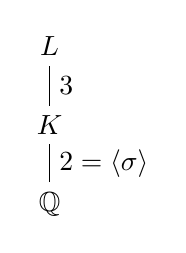
\begin{tikzpicture}
      \node (Q) {$\Q$};
      \node (K) at (0, 1) {$K$};
      \node (L) at (0, 2) {$L$};
      \draw (Q) -- (K) node [pos=0.5, right] {$2 = \bra \sigma\ket$};
      \draw (K) -- (L) node [pos=0.5, right] {$3$};
    \end{tikzpicture}
  \end{center}
  then $K$ is one of $\Q(\sqrt{5})$, $\Q(\sqrt{-7})$ and $\Q(\sqrt{-35})$. We then want $L/K$ to cyclic of degree $3$, and $\sigma$ must act non-trivially, or else we get an abelian extension instead.

  The subgroup $U \subseteq J_K$ corresponding to $L$ msut have $(J_K: U) = 3$, and $U \supseteq \mathcal{O}_v^\times$ for all $v \nmid 35$. We also need $\sigma(U) = U$, or else the extension would not even be Galois, and $\sigma$ acts as $-1$ on $J_K/U \cong \Z/3\Z$.

  We consider the various cases in turn.
  \begin{itemize}
    \item If $K = \Q(\sqrt{-7})$, then this has class number $1$, and the units are $\pm 1$. Soo we know
      \[
        \frac{C_K}{C_K^0} = \frac{\hat{\mathcal{O}}_K^\times}{\{\pm 1\}}.
      \]
      Since $U$ contains $\prod_{v \nmid 35} \mathcal{O}_v^\times$, we are only interested in the places that divide $35$. We see that $5$ is inert in $K$ and $7$ is ramified.

      Since $5$ is inert, we know $K_5/\Q_5$ is an unramified quadratic extension. So
      \[
        \mathcal{O}_{(5)}^\times = \F_{25}^\times \times (1 + 5\mathcal{O}_{(5)})^\times.
      \]
      The second factor is a pro-5 group, and so it must be contained in $U$.for the quotient to have order $3$. On $\F_{25}^\times$, $\sigma$ acts as the Frobenius $\sigma(x) = x^5$. Since $\F_{25}^\times$ is cyclic of order $24$, there is a unique index $3$ subgroup, say $U_5 \subseteq \mathcal{O}_{(5)}^\times$, and on it, $\sigma$ acts by $x \mapsto x^5 = x^{-1}$. This completes the analysis of the prime $5$.

      Since $7$ is ramified, we have
      \[
        \mathcal{O}_{(\sqrt{-7})}^\times = \F_7^\times \times \left(1 + (\sqrt{-7}) \mathcal{O}_{\sqrt{-7}}\right)^{\times},
      \]
      and the second factor is a pro-$7$ group. Now $\sigma$ acts trivially on $\F_7^\times$. This tells us $U$ must contain $\mathcal{O}_{(\sqrt{-7})}^\times$.

      So we must have
      \[
        U = \prod_{v \not= (5)} \mathcal{O}_v^\times \times U_5.
      \]
      So there is exactly one $L$ containing $\Q(\sqrt{-7})$. Exercise: find an explicit polynomial for this.
    \item The remaining cases are exercises.
  \end{itemize}
  We see that there are no more.
\end{eg}

\printindex
\end{document}
